% !TEX root = Master.tex


After World War II, the \textit{"Dassler Brothers Shoe Factory"} (German: \textit{"Gebrüder Dassler Schuhfabrik"}), which was led by \textit{Adolf Dassler} (aka \textit{Adi Dassler}) and his brother Rudolph, was dissolved. The brothers split up and formed their own firms. As a result, the sports shoe factory \textit{"Adi Dassler adidas Sportschuhfabrik"} was founded on August 18th 1949 by Adolf Dassler in Herzogenaurach, a small town in Germany \citep{adidas-group}.

\begin{figure}[H]
\centering
\begin{subfigure}{.4\textwidth}
  \centering
  
\includegraphics[width=\linewidth]{figures/adidas_performance_logo.eps}
  \caption{adidas Performance}
  \label{fig:adidas_performance_logo}
\end{subfigure}
\begin{subfigure}{.4\textwidth}
  \centering
  
\includegraphics[width=\linewidth]{figures/adidas_originals_logo.eps}
  \caption{adidas Originals}
  \label{fig:adidas_originals_logo}
\end{subfigure}
\caption{Two of the adidas-group logos: Performance (left) \& Originals (right) \\ \citep{adidasmediacenter}}
\label{fig:adidas_logos}
\end{figure}


Today, just over 70 years later, the sportswear designer and manufacturer is known as the \textit{"adidas AG"} (short: \textit{adidas}) and is one of the world's biggest sports and fashion brands. The global headquarters of are located in the birthplace Herzogenaurach and the company is employing over 59,000 people worldwide, with \textit{Kasper R\o rsted} leading the brand as CEO since October 1st 2016. In 2019, adidas produced over 1.1 billion sports and sports lifestyle products and is nowadays sponsoring a vast range of athletes, artists and organizations across the globe (e.g. the  \href{https://www.fifa.com/worldcup/}{FIFA World Cup\texttrademark}).

\begin{figure}[H]
\centering
  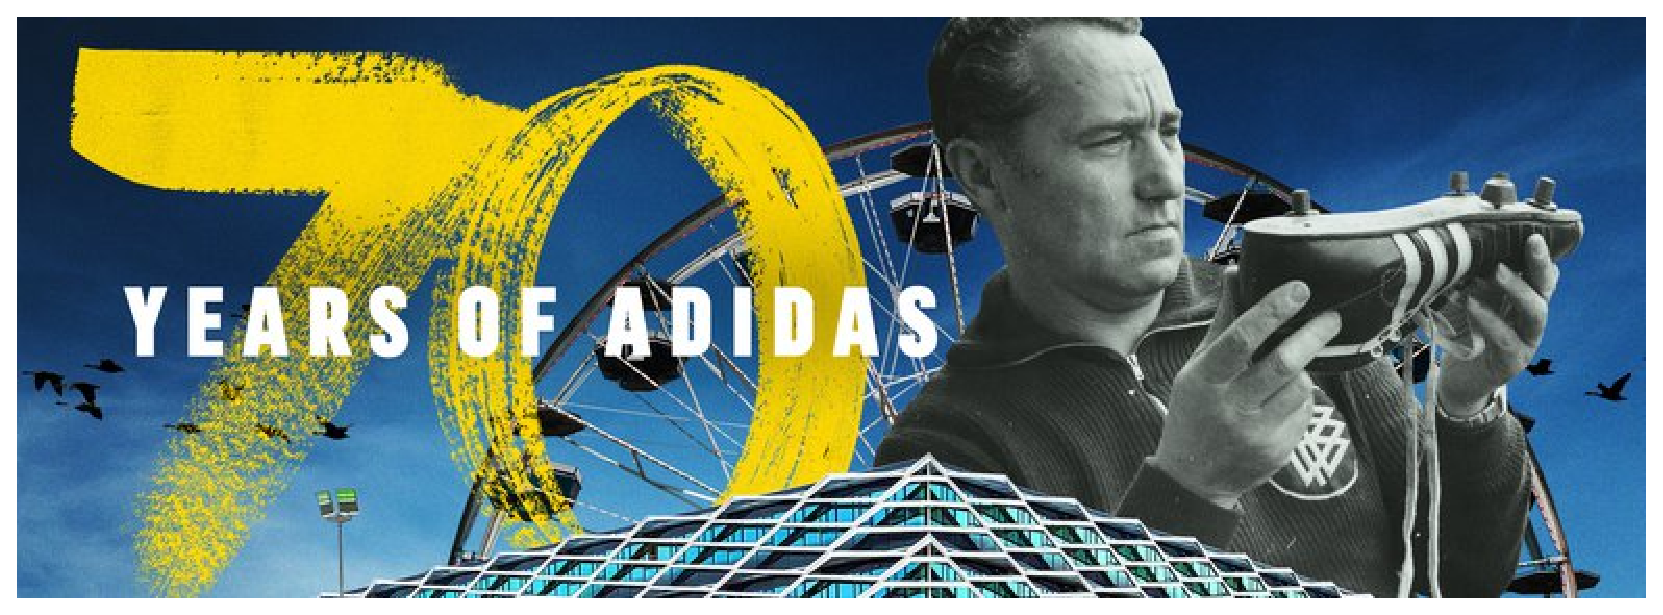
\includegraphics[width=.95\linewidth]{figures/adidas_70_years.eps}
  \caption{adidas celebrates its 70th anniversary and the opening of the ARENA building \citep{adidas70years}}
  \label{fig:adidas_70_years}
\end{figure}


More on  DNA, DS\&AI, etc...?